\documentclass[a4paper,oneside,12pt]{article}

\usepackage[american]{babel}

\usepackage{graphicx}
\usepackage{listings}

% figure counter???
%\usepackage{chngcntr}
%\counterwithout{figure}{chapter}
%\counterwithout{figure}{section}

%\setcounter{figure}{0}
%\renewcommand{\thefigure}{\arabic{section}.\arabic{figure}}

\newcommand{\half}{\frac{1}{2}}
\newcommand{\dt}{\Delta t}

% better tables
\usepackage{multirow}
\usepackage{booktabs}

% links
%\usepackage{color}
\usepackage[]{hyperref}
%bibliography
\usepackage[backend=biber,
style=numeric,
sorting=none,
natbib=true,
babel=other,
bibencoding=auto,
language=autobib,
giveninits=true]{biblatex}
% figures and tables
% \usepackage{caption}
% \captionsetup[figure]{labelfont=it,textfont=it}
% \captionsetup[table]{labelfont=it,textfont=it}
% \usepackage{subfig}

%%\usepackage[strict]{changepage}
% Define margins
%%\usepackage[left=2.5cm,right=2.5cm,top=2.5cm,bottom=2.5cm,includehead,includefoot,headheight=16pt]{geometry}

% Page headers
\usepackage{fancyhdr}
\fancyhf{}
\renewcommand{\headrulewidth}{0pt} 
\fancyhead[L]{\nouppercase{\leftmark}}
\cfoot{\thepage}
\pagestyle{fancy}


% Line spacing
%\usepackage{setspace}
%\setstretch{1.5}

% Defines uth-specific title page
%\usepackage{mieUTHtitle-en}
\usepackage{pgfplots} 
\usepackage{algorithm}
\usepackage{algpseudocode}

%Correct spelling of words. If the spelling of a word is incorrect and LaTex puts a hyphen at the wrong place on a line break then we give the correct spelling here.
%\babelhyphenation[greek]{Anti-here}
%-------------------------------------------

\begin{document}

% Fill in your details
\author{Alexander Pletzer, Chris Scott (NeSI/REANNZ), \\
Inna Senina, Lucas Bonnin and Romain Forestier (SPC)}
\title{Implementation of cohort parallelisation in the Seapodym code}

\maketitle

\begin{abstract}
This report describes NeSI/REANNZ's consultancy project entitled ``SEAPODYM cohort parallelisation'' 
whose work was performed from May to September 2025. The outcome of this work is a C++ library,
\verb|seapodym-parallel|, which can be leveraged by the SEAPODYM code to parallelize the spatio-temporal
evolution of tuna fish densities in the Pacific. The \verb|seapodym-parallel| library implements a 
variation of the manager/worker setup whereby workers create new fish age cohorts and advances these in time. 
The manager distributes tasks to the workers and stores results. The implemented manager/worker design differs from 
traditional implementations in that tasks can only be started when other tasks have completed specific internal steps. 
\end{abstract}

%\frontmatter

\pagestyle{plain}


\section{Statement of the problem}

SEAPODYM is a quantitative spatio-temporal model
of population dynamics that solves partial differential
equations with initial and boundary conditions in C++. 
The model is parameterized using a maximum
likelihood estimation approach that integrates georeferenced 
datasets obtained from industrial fishing and scientific campaigns.

The objective of this work is to parallelise the SEAPODYM code over cohorts. 
This was achieved by designing and implementing the sepodym-parallel library 
(\url{github.com/PacificCommunity/seapodym-parallel.git}), a collection of 
C++ classes that abstract parallelization. This library comes with a 
\verb|CMake| build system, unit tests and continuous integration via 
GitHub actions. The documentation of the API can be found at 
\url{https://pacificcommunity.github.io/seapodym-parallel/}.


A cohort is a group of fish that are born at the same time. Each cohort 
can be integrated forward in time independently of other cohorts, until the cohort reaches a certain age and dies. 
At the next time step, a new cohort is born and integrated forward in time until it dies. Except 
at the first time step, the initial condition of each cohort depends on 
the density of the other cohorts at the previous time step. Thus, the integration of 
each cohort must take into account the state of the other cohorts and this requires 
careful consideration when parallelising the code.

An example of cohort time integration is shown below:
\begin{equation} \label{eq:cohorts}
\begin{array}{ccc}
0 & 1 & 2 \\
3 & 1 & 2 \\
3 & 4 & 2 \\
3 & 4 & 5 \\
6 & 4 & 6 \\
6 & 7 & 6
\end{array}
\end{equation}
Here, the vertical axis represents time increasing from top to bottom ($N_t = 6$). The horizontal axis represents the 
tasks than can be performed concurrently. Each row represents different age groups ($N_a = 3$). 
Each cohort is identified by an integer ($0, 1, \cdots 7$). 

Cohort 1 is one unit time older than cohort 2. Therefore cohort 1 dies one time step before cohort 2. 
The number of time steps 
a cohort is integrated is $i = i_{beg} \cdots i_{end} - 1$ where $i_{beg} \geq 0$  and $i_{end} <= N_a$. In our example, we have
\begin{table}[htbp]
    \centering % Centers the table horizontally
    \caption{Start and end integration indices for each cohort}
    \label{tab:cohort_indices}
    \begin{tabular}{c|cc} % Three centered columns
        \toprule % Top rule (from booktabs)
        cohort Id & $i_{beg}$ & $i_{end}$ \\
        \midrule % Middle rule (from booktabs)
        0 & 2 & 3 \\
        1 & 1 & 3 \\
        2 & 0 & 3 \\
        3 & 0 & 3 \\
        4 & 0 & 3 \\
        5 & 0 & 3 \\
        6 & 0 & 2 \\
        7 & 0 & 1 \\
        \bottomrule % Bottom rule (from booktabs)
    \end{tabular}
\end{table}
When a cohort dies, it is replaced by a new cohort at the next time step. To instantiate the new cohort, data will need 
to be communicated from the cohorts at the previous time step. Figure \ref{fig:cohort_deps} shows the dependency of the new cohorts on the older 
cohorts at different steps.
\begin{figure}[htbp]
    \centering
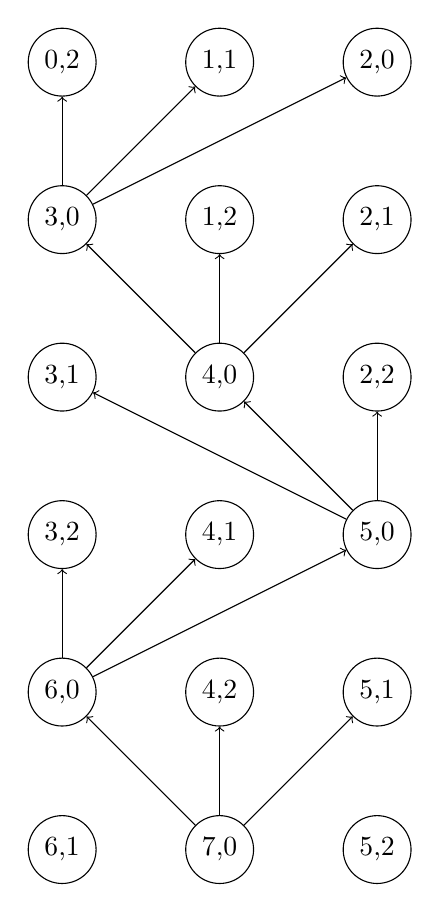
\begin{tikzpicture}[main/.style = {draw, circle}, node distance=2cm]
    \node[main] (02) {0,2};
    \node[main] (11) [right of= 02]{1,1};
    \node[main] (20) [right of= 11]{2,0};

    \node[main] (30) [below of= 02]{3,0};
    \node[main] (12) [right of= 30]{1,2};
    \node[main] (21) [right of= 12]{2,1};

    \node[main] (31) [below of= 30]{3,1};
    \node[main] (40) [right of= 31]{4,0};
    \node[main] (22) [right of= 40]{2,2};

    \node[main] (32) [below of= 31]{3,2};
    \node[main] (41) [right of= 32]{4,1};
    \node[main] (50) [right of= 41]{5,0};

    \node[main] (60) [below of= 32]{6,0};
    \node[main] (42) [right of= 60]{4,2};
    \node[main] (51) [right of= 42]{5,1};

    \node[main] (61) [below of= 60]{6,1};
    \node[main] (70) [right of= 61]{7,0};
    \node[main] (52) [right of= 70]{5,2};



    \draw[->] (30) -- (02);
    \draw[->] (30) -- (11);
    \draw[->] (30) -- (20);

    \draw[->] (40) -- (30);
    \draw[->] (40) -- (12);
    \draw[->] (40) -- (21);

    \draw[->] (50) -- (31);
    \draw[->] (50) -- (40);
    \draw[->] (50) -- (22);

    \draw[->] (60) -- (32);
    \draw[->] (60) -- (41);
    \draw[->] (60) -- (50);

    \draw[->] (70) -- (60);
    \draw[->] (70) -- (42);
    \draw[->] (70) -- (51);

\end{tikzpicture}
\caption{Dependency of cohort tasks on other cohort, step tuples. The first digit is the cohort Id and the second the step. }
    \label{fig:cohort_deps}
\end{figure}


\section{Task farming with dependencies on other tasks' steps}

We opted for a task farming approach. This involves creating a pool of tasks that can be executed concurrently
and a manager that assigns the tasks to the workers. Each task consists of advancing a cohort in time.

In classical task farming, the manager starts by assigning tasks to the workers. This involves sending a message to each worker, along with 
some input parameters. Each worker then executes the task and reports the results back to the manager, who then assigns a new task to the worker. 
When no more tasks are available, the manager sends a message to the workers to shut down. Task farming is particularly suitable when tasks 
take a various amount of time to execute.

Clearly, the dependencies between tasks and sub-tasks shown in Fig. \ref{fig:cohort_deps} prevents us from using such a naive task farming approach. 
In our case, tasks can only be started when other tasks' particular steps have completed
(as indicated by the arrows in Fig. \ref{fig:cohort_deps}). This requires the manager to keep track of task-step dependencies.

We start by describing a worker's task. A worker waits for a task to be assigned by the manager. A task has a identification number \verb|taskid| 
that fully describes the task to accomplish. The worker reports back the status of the execution of each task to the manager. 
The corresponding pseudo-code is shown in Algorithm \ref{algo:worker}.

\begin{algorithm}
\caption{A worker's pseudo-code.}
    \begin{algorithmic}[1] % [1] for line numbering
    \While {true}

        taskid = \Call{getTaskIdFromManager}{};
        \If {taskid $< 0$}
            Break
        \EndIf

        \Comment{Perform the task, stepping from stepBeg to stepEnd - 1}   
        \State \Call{taskFunc}{taskid, stepBeg, stepEnd}

        \Comment{Notify the manager that this worker is available again}
        \State \Call{sendSignalToManager}{DONE}
    
    \EndWhile
\end{algorithmic}
\label{algo:worker}
\end{algorithm}

The task function defined in Algorithm \ref{algo:worker} is responsible for advancing the cohort associated with \verb|taskid| from \verb|stepBeg| to \verb|stepEnd - 1|.
\begin{algorithm}
\caption{The task function executed by the worker.}
    \begin{algorithmic}[1] % [1] for line numbering
\Function{MyFunction}{taskid, stepBeg, stepEnd}
    \State data = \Call{getDataFromManager}{taskid}
    \State cohort = \Call{createCohort}{taskid}
    \Comment{Advance a cohort}
    \For {step = stepBeg to stepEnd - 1}
        \State \Call{stepForward}{cohort}
        \State \Call{sendStepCompleteMessageToManager}{taskid, step}
    \EndFor
\EndFunction
\end{algorithmic}
\label{algo:worker}
\end{algorithm}
Note the call to \verb|sendStepCompleteMessageToManager| which informs the manager that a specific step for a task has been completed. 
This is crucial for managing task dependencies.

The manager code orchestrates the work. It maintains a list of all active workers, a task queue, a list of completed tasks and stores the results. 
Since workers will be sending various types of messages (``worker is available'' or ``result of task-step X''), the manager needs to be able to 
distinguish between them. This is done using message tags.
The manager's pseudo-code is shown in Algorithm \ref{algo:manager}.

\begin{algorithm}
\caption{The manager's pseudo-code.}
    \begin{algorithmic}[1] % [1] for line numbering

    \While{not taskQueue.empty() or  not assigned.empty()}

        \Comment{Look for messages ``task-step complete''}
        \While{true}

            \Comment{Probe for messages from workers}
            \State msg = getMessageFromAnyWorker{}
            \If{msg.type != ``task-step complete''} 
              \State break
            \EndIf

            \Comment{Store the result}
            \State results.insert{msg.output}
            \State taskid = output[0]
            \State step = output[1]
            completed.insert{taskid, step}

            \If{step == stepEnd - 1}
                assigned.erase{taskid};
            \EndIf
        \EndWhile

        \Comment{Assign ready tasks to any available worker}    
        \For{taskid in taskQueue}
            \State taskDependencies = getTaskStepDependencies{taskid}
            \State bool ready = true
            \For{dep in taskDependencies}
                \If{completed.find{dep} == completed.end{}}
                    \State ready = false
                    \State break
                \EndIf
            \EndFor
            \If{ready and !activeWorkers.empty{}}
                \State worker = activeWorkers.begin{}
                \State activeWorkers.erase{worker}
                \State \Call{sendTaskToWorker}{taskid, worker}
                \State assigned.insert{taskid}
                \State taskQueue.erase{taskid}
            \EndIf
        \EndFor

        \Comment{Drain all worker-available messages}
        \For{worker in workers}
            \State msg = getMessageFromAnyWorker{}
            \If{msg.type == ``worker is available''}
                \State activeWorkers.insert(worker)
            \EndIf
        \EndFor

    \EndWhile

    \Comment{Send stop signal to workers}
    \State stop = -1
    \For{worker in workers}
        \Call sendStopSignalToWorker{worker}
    \EndFor

\end{algorithmic}
\label{algo:manager}
\end{algorithm}

\section{Scalability}

\begin{figure}
    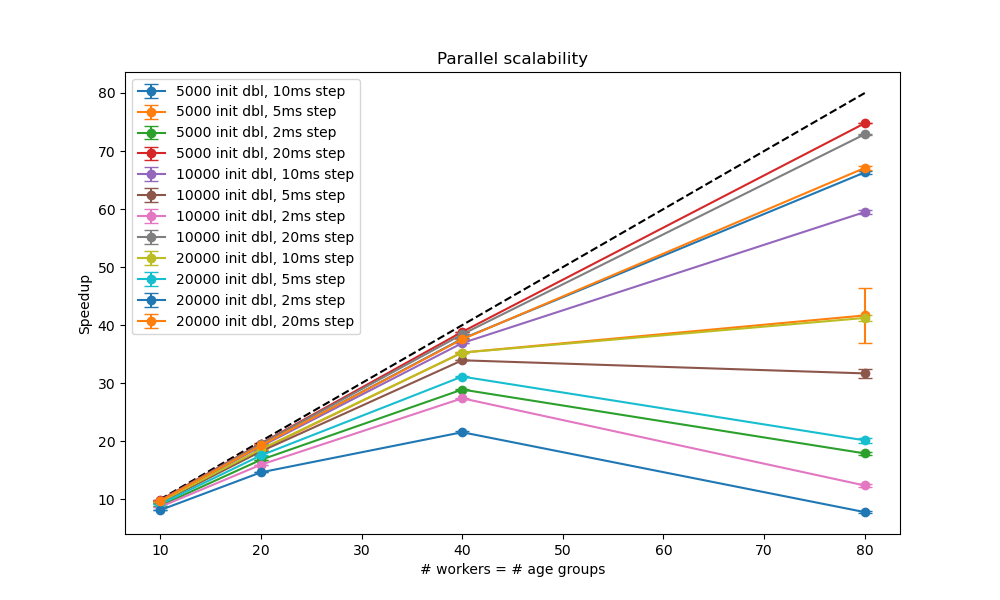
\includegraphics[width=15cm]{results/speedup_vs_workers.png}
    \caption{Parallel scalability for different step execution 
    times and number of doubles initially fetched from the manager. 
    The number of age groups matches the number of workers. These results 
    assume no initialisation setup time.}
    \label{fig:speedup}
\end{figure}

Figure \ref{fig:speedup} shows the parallel scalability of the cohort parallelisation 
approach described above as the number of workers is increased (see code \verb|testTaskStepFarmingCohort|). 
The speedup numbers were obtained for an idealized scenario, assuming 
a fixed cost of communication to initialize a new cohort and a constant cost of executing a step
on the NeSI/REANNZ AMD Milan node cluster.
In all cases the number of workers was chosen to match the number of age groups $N_a$.

Perfect parallel scaling 
is shown as the black dashed line. Good scalability depends on the time taken to execute 
each step and the amount of data fetched from the manager at the start of each task. Parallel 
efficiency $> 50\%$ is achieved for time step times $\geq 10$ms and initial data sizes 
$\leq 10000$ doubles. For instance, a time step taking $10$ms and an initial data size of 
$10000$ doubles gives a speedup of 60, when using $80$ workers, i.e. $75\%$ parallel efficiency.

Note that at every step the worker sends data to the manager, as well as a message 
to inform the manager that the step has been completed. This introduces a communication overhead
that limits parallel scalability. 
Taking the example of $20,000$ doubles sent by 80 workers to the manager at a cadence of 
 $10$ms, we get a data transfer rate of $1.3$GB/s = $100$Gb/s, which is close to the bandwidth 
 of the Infiniband communication fabric. To further improve parallel scalability, one would need to 
 either increase the computational load per step, reduce the amount of data to be transferred or apply
some form of data compression. For instance, one could send floats instead of double and this would 
improve the speedup from 40 to 60. 

\section{The cost of initialization}

Scalability can be affected by load balancing. Some concurrently executed tasks may take longer than others
to complete. When synchronization occurs, which is the case at every time step in Seapodym, then 
workers whose task has finished need to wait for the slowest woprker to finish their task. While the evolution of
the reaction-diffusion equations takes the same time for all cohorts, the initialization of a new cohort, which occurs
at every time step, can lead to severe load imbalance and can thus affect the parallel speedup. 
Fig. \ref{fig:c2i} shows the the ratio of the compute time over the initialization time, the higher the 
better. Initialization involves reading data from file and other one off operations. 

There are different ways to amortize the high cost of initialization. One possibility is to avoid constructing a new 
cohort at every time step. Instead a ``vanilla'' cohort is created initially, when the simulation start. This cohort,
reads the restart files, the input files and set things up. Only the final stage of the construction, which 
involves reading forcing data and spawning, is executed when launching the new cohort. 


\begin{figure}
    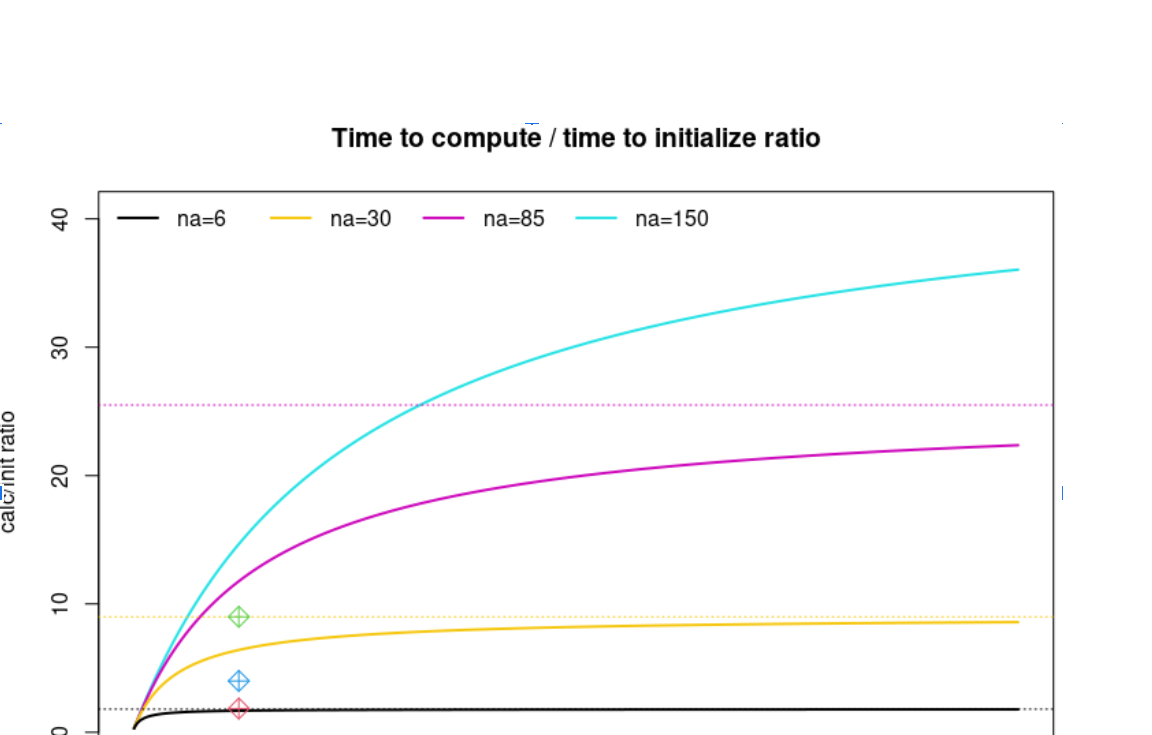
\includegraphics[width=15cm]{c2i.png}
    \caption{Ratio of compute over initialization time for Seapodym.}
    \label{fig:c2i}
\end{figure}

\section{Comparing blocking and non-blocking get operations}

A significant part for the initialization time involves fetching data from the manager. 
Our library support asynchronous get operations, which allow one to 
overlap communication with computation. 

The default mode to \verb|get| data is blocking, that is the retrieved data are ready when the call
completes. Alternatively, the programmer may rely on \verb|getAsync| calls. In this case the programmer 
indicates his/her desire to fetch the data but the data need not be immediately available. A \verb|startEpoch|
and \verb|endEpoch| calls around the \verb|getAsync| operations determine the time interval 
when remote memory access operations take place. The retrived data are guaranteed to be available only when
\verb|endEpoch| is called. (An additional ``flush'' medthod can be invoked
to synchronize operations within a period.)

In Fig. \ref{fig:async} we compare the  execution time of MPI \verb|get| operations using 
the blocking and non-blocking variants. Each test (implemented in \verb|testAsyncPutGet|) involves reading $N$ chunks ($=$ number of workers) 
of $nd$ values from rank 0 and summing the result. In the blocking test, the chunks are read one at a 
time, followed by a sleep operation lasting $nm$ milliseconds and a sum operation over the chunk. 
In the nonblocking test, a big array is filled by reading the chunks asynchronously, followed by the 
sleep operation -- these two operations are within a single epoch. The final step then involves summing up the values
of the big array. The benefit of using non-blocking \verb|get| calls is particulalry apparent for large chunks 
$nd$ and small amount of work (low $nm$).

\begin{figure}
\begin{tabular}{|c|c|}
      % after \\: \hline or \cline{col1-col2} \cline{col3-col4} ...
      \includegraphics[width=60mm]{speedup_async_N20.png} & \includegraphics[width=60mm]{speedup_async_N40.png} \\
      \includegraphics[width=60mm]{speedup_async_N80.png} & \includegraphics[width=60mm]{speedup_async_N160.png} \\
\end{tabular}
\label{fig:async}
\end{figure}


\section{Summary and future work}
   

\end{document}